% !TeX root = ../thuthesis-example.tex

\chapter{简介}

\section{历史背景}

\begin{figure}[h]
\center
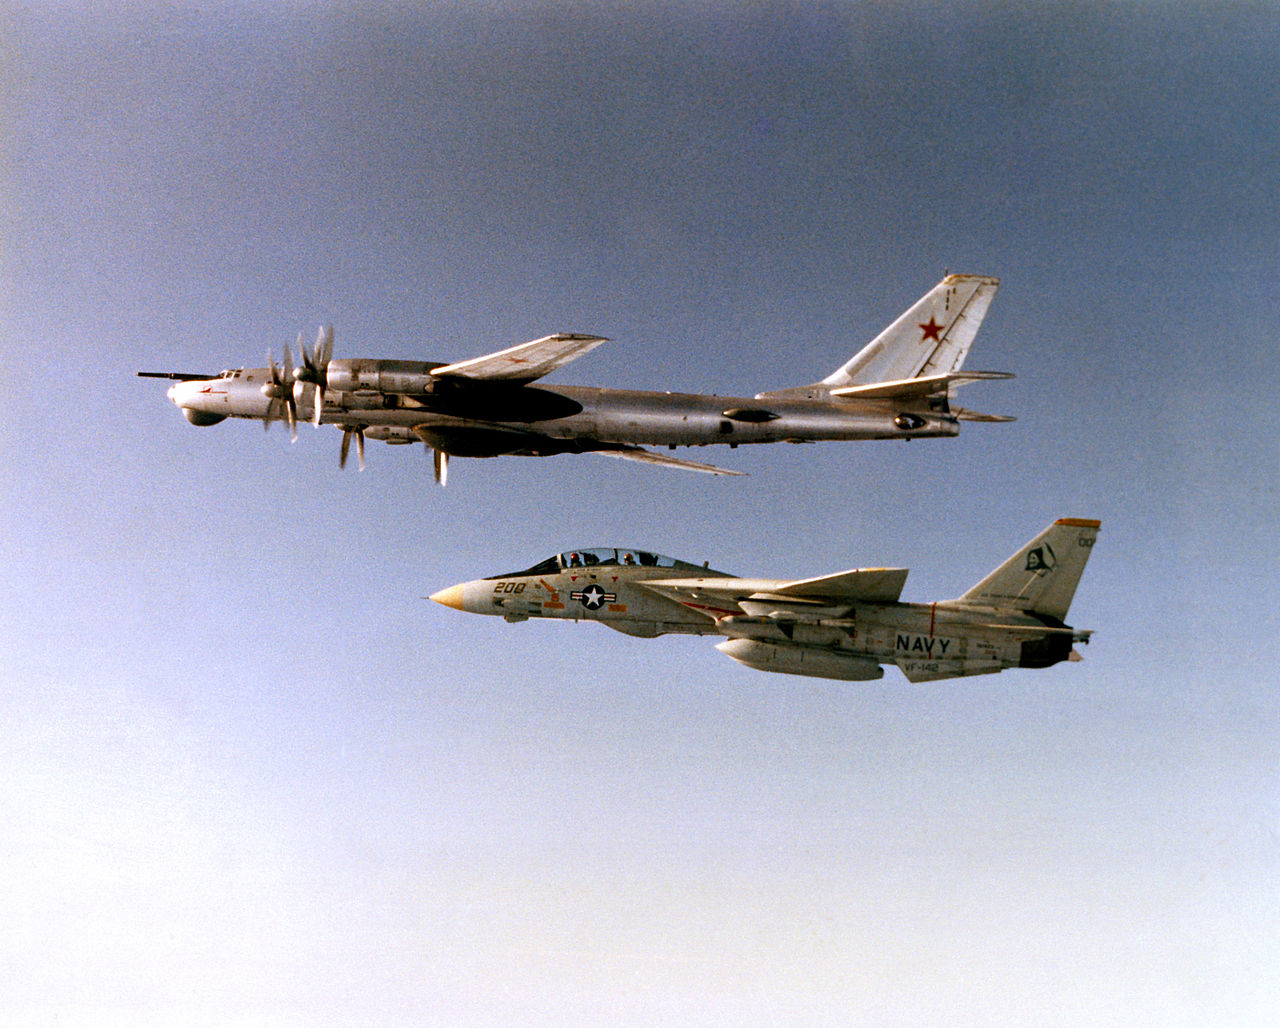
\includegraphics[width=0.6\textwidth]{F-14TU95.png}
\caption{照片由美国海军中尉Thomas Prochilo拍摄(DN-SC-83-06680)}
\end{figure}

F-14“雄猫”可以一直追溯到上世纪50年代,美国海军急需一架长航程舰载截击机来填补舰队防空职能的空缺。结论认为海军需要一架比 F-4“鬼怪”更先进、雷达探测距离更远、空空导弹射程更长的战斗机。

当时,海军受国防部长罗伯特·麦克纳马拉的指示与美国空军合作推进实验战术战斗机(TFX)项目。海军从最初便反对共同开发此项目,而且通用动力F-111B飞机方案也并未满足海军的期望。

和通用动力共同开发海军 F-111B 而加入 TFX 项目的格鲁曼公司最终获得了海军制定的更符合自身情况的舰载机研发合同。装备着沿用失败的 F-111B 项目的雷达(AN/AWG-9)和导弹(AIM-54“不死鸟”)的 F-14 战斗机便从这份研发合同中诞生了。

F-14“雄猫”于1970年12月21日首飞,并于1974年9月22日开始服役。“雄猫”(Tomcat)这个名字一方面遵循格鲁曼用猫科动物命名飞机的传统,另一方面也源于海军中将Thomas F. Connolly的昵称“Tom's Cat”(“汤姆的猫”),以纪念他对F-14研发所做的关键贡献。

\subsection{服役升级}

F-14A是F-14战斗机的第一个型号,配备普惠TF30发动机并在机鼻下方的吊舱中装备了IRST系统。

对 F-14A 而言,TF30 发动机的稳定性和动力常常不尽人意。于是在 F-14A+(后来的 F-14B )上,TF30发动机被通用电气 F110-400 发动机所取代。

F-14A 的 IRST 系统也表现不佳并很快被 TCS(电视摄像机组件)吊舱所取代。TCS 吊舱允许飞行员对雷达追踪目标进行超视距目视识别。

F-14A 和 F-14B 在服役期间都得到了持续升级,包括新的可编程座舱显示器(PTID 和 PMDIG),以及新的 INS 惯导系统、数字飞控系统(DFCS)和 RWR 系统等。

最终,TARPS(战术空中侦察吊舱)系统的装备使 F-14 获得了收集影像资料进行战术侦查任务的能力。

\subsection{对地攻击}

\begin{figure}[h]
\center
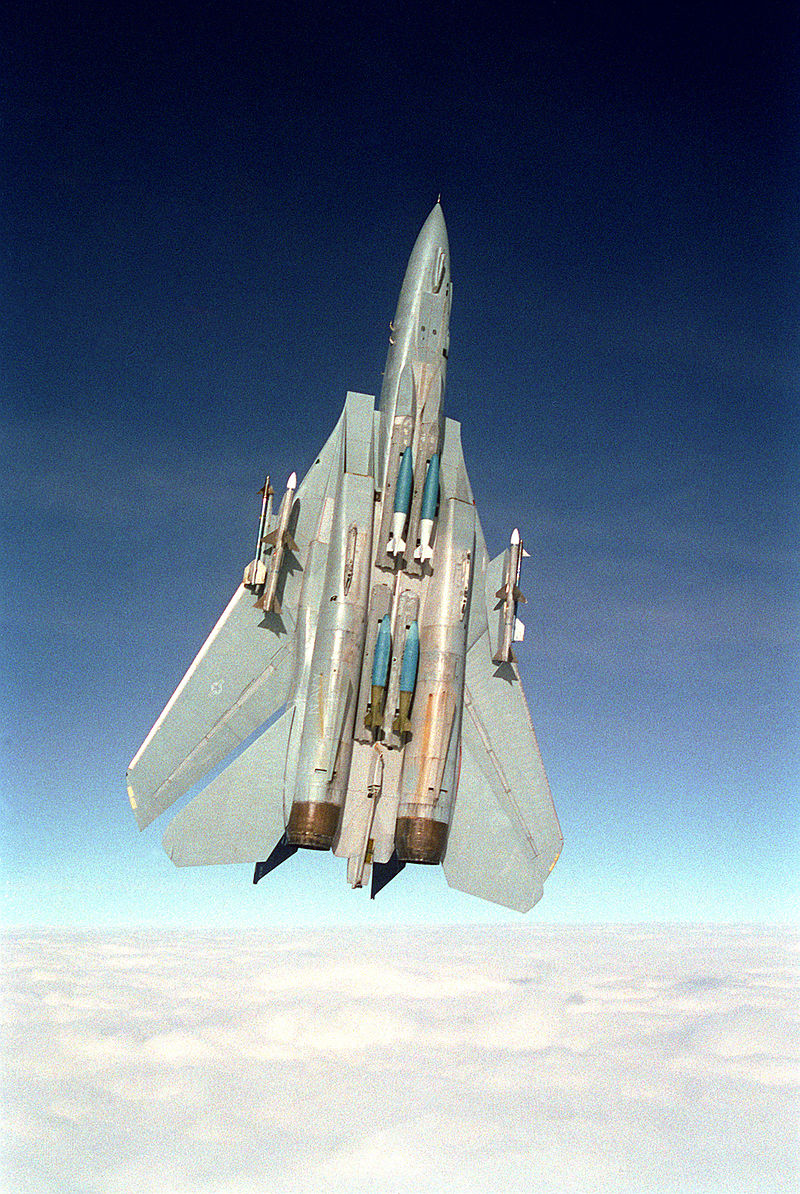
\includegraphics[width=0.6\textwidth]{bombcat.png}
\caption{照片由美国海军少校 Dave Parsons 拍摄 (DN-SC-93-01299)}
\end{figure}

20世纪90年代,美国海军舰队面临的空中威胁逐渐减少,同时由于沙漠风暴等行动的实施,对地攻击的重要性重新凸显出来。

F-14 最初就具备携带和投放空对地弹药的能力,但是由于海军基于成本和风险的考量,F-14 的主要职责仅为舰队防空。

随着任务角色的转变,一些 F-14A 和 F-14B 开始挂载 LANTIRN 目标吊舱以便 RIO 为自己和其他飞机搜索目标、引导激光制导炸弹。 随后,F-14 还增加了携带和投放 GPS 制导的 JDAM 弹药的能力。

大部分装备了 LANTIRN 吊舱的 F-14 都升级了可编程 TID(PTID)以更好地集成 LANTIRN 吊舱的功能。

\subsection{F-14D}

20世纪90年代,F-14 的终极型号 F-14D 开始服役。

F-14D 使用和 F-14B 同样的 GE F110-400 发动机,同时也装备了数字飞控系统(DFCS)。DFCS 系统随后也开始装备在较老的在役 F-14A 和 B 型上。

此外,F-14D 还安装了 AN/AWG-9 雷达的改进型,AN/APG-71 雷达以及一整套升级的航电系统。原本的 TCS 吊舱也升级成了一个融合了改进版 IRST 系统与 TCS 功能的新吊舱。

\subsection{退役}

F-14“雄猫”最终还是老态龙钟了。随着维护成本的增加和机体的老化,海军不得不开始退役“雄猫”。冷战的结束也使得“雄猫”的本职——舰队防空显得不那么重要了。

2006年9月22日,最后一架雄猫的退役仪式在欧希安纳海军航空站举行。

\subsection{伊朗}

\begin{figure}[h]
\center
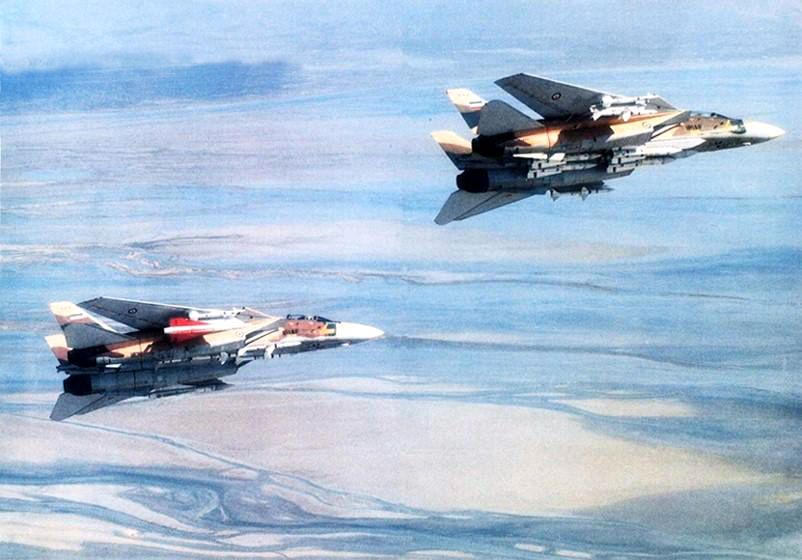
\includegraphics[width=0.6\textwidth]{iranicats.jpg}
\caption{照片由伊朗空军在1986年间拍摄}
\end{figure}

F-14“雄猫”的唯一海外使用客户是伊朗皇家空军(IIAF)和后来的伊朗伊斯兰共和国空军(IRIAF)。当时的伊朗国王默罕默德·礼萨·巴列维曾采购了80架“雄猫”。

而巴列维王朝的倒台和伊朗伊斯兰共和国的崛起意味着一个反美国家获得了美国最先进的战斗机之一。“波斯猫”随即失去了所有零部件和导弹的供应,只得从黑市上购买配件,这大大增加了飞机维护的难度。

伊朗在两伊战争期间使用了 F-14“雄猫”并声称取得了大量对伊拉克空军的空中胜利。小道消息称当时伊拉克飞行员甚至会为了避开 AN/AWG-9 和 AIM-54 的威胁而逃离交战空域。

目前为止,只有伊朗共和国空军还在使用 F-14“雄猫”。目前伊朗人获得飞机配件的途径还不明确,有推测认为他们通过拆除无法飞行的飞机上的零件来维持机队其他飞机的状态。还有传言说他们通过黑市和土法自产一些零件以供使用。

伊朗使用的“雄猫”是早期 F-14A 的改进版,使用 TF30 发动机,没有装备 TCS 或者 IRST 系统。

\subsection{AIM-54"不死鸟"}

\begin{figure}[h]
\center
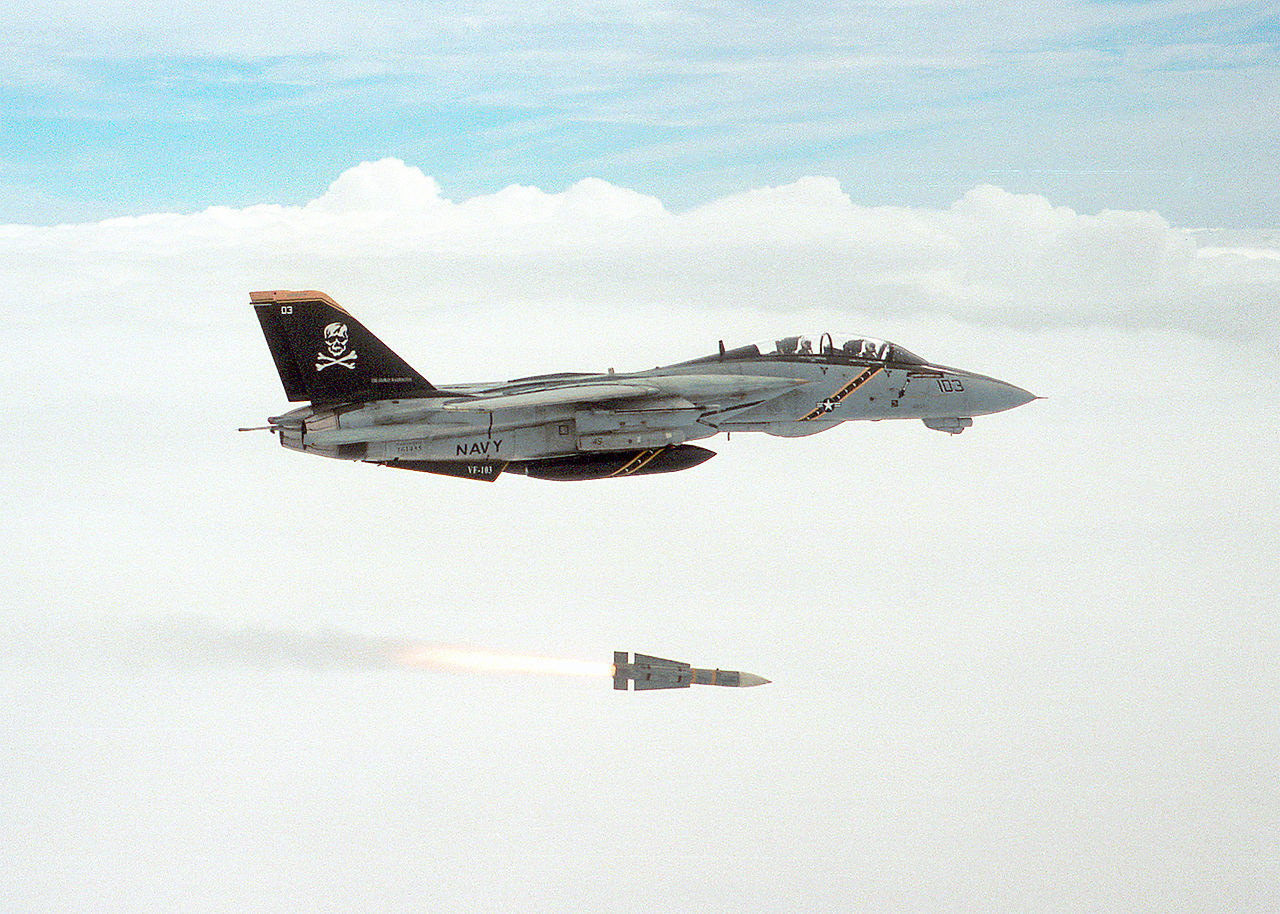
\includegraphics[width=0.6\textwidth]{phoenix.jpg}
\caption{照片由美国海军上尉 Dana Potts 拍摄 (020924-N-1955P-001)}
\end{figure}

AIM-54 远程空空导弹和F-14“雄猫”一起诞生于当年的TFX项目。

最初为 F-111B 设计的 AIM-54 被 F-14 用作可以同时攻击敌方轰炸机和巡航导弹的长射程导弹。当然,AIM-54 打击其他小目标也并非力不从心。

AIM-54 导弹最突出的特点便是超远的射程。AIM-54 还具有同时发射和跟踪最多6个目标的能力,先由载机上的 AN/AWG-9 雷达制导,然后用自己的主动雷达引导头独立制导。

AIM-54 最初的型号是安装 Mk47火箭发动机的 AIM-54A。Mk47 发动机后来升级为 Mk60 火箭发动机以增加导弹的射程。而 AIM-54 本身也经过升级成为 AIM-54C,改进的引导头引导能力更强,新的 Mk47 发动机发烟量也更少,更难被目视发现。

美国海军在实战中仅发射了3枚 AIM-54 导弹,均于伊拉克上空发射。3枚导弹都没有击中目标,其中2枚由于火箭发动机失效,第三枚则是目标自己掉头逃跑而未能命中。

不为西方所知的是,IRIFA则宣称使用 AIM-54 对伊拉克的米格-21、米格-23、米格-25、幻影F-1和超军旗等飞机获得了至少78次空中胜利,战果甚至还包括了数枚反舰巡航导弹。

\section{一般规格}

\begin{table}[htbp]
  \centering
  \caption{F-14B 技术资料}
  \begin{minipage}[t]{0.8\textwidth}
    \begin{tabularx}{\linewidth}{|l|X|X|X|X|}
      \hline
      翼展(机翼完全展开)& 64'1.5"(约19.5米)\\
      \hline
      翼展(空中完全后掠) & 38'2.5"(约11.6米)\\
      \hline
      翼展(停放机翼后掠)& 33'3.5"(约10.1米)\\
      \hline
      长度 & 62'8.5"(约19.1米)\\
      \hline
      高度 & 16' (约4.9米)\\
      \hline
      翼面积 & 565平方英尺(约52.5平米)\\
      \hline
      空重 & 41,780磅(约19,000千克)\\
      \hline
      最大重量 & 74,349磅(33,700千克)\\
      \hline
      加力最大推力 & 60,400磅力(268千牛顿)\\
      \hline
      翼载 & 94磅/平方英尺(458.9千克/平方米)\\
      \hline
      极速 & 1,544英里/小时(~2,500千米/小时)\\
      \hline
      升限 & 53,000+英尺(~16,200米)\\
      \hline
      航程 & 2,050海里(~3,800千米)\\
      \hline
    \end{tabularx}\\[2pt]
  \end{minipage}
\end{table}

% \chapter{带 English 的标题}
% \label{cha:intro}

% 这是 \thuthesis\cite{thuthesis} 的示例文档,基本上覆盖了模板中所有格式的设置。建
% 议大家在使用模板之前,除了阅读《\thuthesis{} 用户手册》,这个示例文档也最好能看一
% 看。

% 小老鼠偷吃热凉粉;短长虫环绕矮高粱\footnote{韩愈(768-824),字退之,河南河阳(
%   今河南孟县)人,自称郡望昌黎,世称韩昌黎。幼孤贫刻苦好学,德宗贞元八年进士。曾
%   任监察御史,因上疏请免关中赋役,贬为阳山县令。后随宰相裴度平定淮西迁刑部侍郎,
%   又因上表谏迎佛骨,贬潮州刺史。做过吏部侍郎,死谥文公,故世称韩吏部、韩文公。是
%   唐代古文运动领袖,与柳宗元合称韩柳。诗力求险怪新奇,雄浑重气势。}。


% \section{封面相关}
% 封面的例子请参看 \texttt{cover.tex}。主要符号表参看 \texttt{denotation.tex},附录和
% 个人简历分别参看 \texttt{appendix01.tex} 和 \texttt{resume.tex}。里面的命令都很直
% 观,一看即会\footnote{你说还是看不懂?怎么会呢?}。

% \section{字体命令}
% \label{sec:first}

% 苏轼(1037-1101),北宋文学家、书画家。字子瞻,号东坡居士,眉州眉山(今属四川)人
% 。苏洵子。嘉佑进士。神宗时曾任祠部员外郎,因反对王安石新法而求外职,任杭州通判,
% 知密州、徐州、湖州。后以作诗“谤讪朝廷”罪贬黄州。哲宗时任翰林学士,曾出知杭州、
% 颖州等,官至礼部尚书。后又贬谪惠州、儋州。北还后第二年病死常州。南宋时追谥文忠。
% 与父洵弟辙,合称“三苏”。在政治上属于旧党,但也有改革弊政的要求。其文汪洋恣肆,
% 明白畅达,为“唐宋八大家”之一。  其诗清新豪健,善用夸张比喻,在艺术表现方面独具
% 风格。少数诗篇也能反映民间疾苦,指责统治者的奢侈骄纵。词开豪放一派,对后代很有影
% 响。《念奴娇·赤壁怀古》、《水调歌头·丙辰中秋》传诵甚广。

% {\kaishu 坡仙擅长行书、楷书,取法李邕、徐浩、颜真卿、杨凝式,而能自创新意。用笔丰腴
%   跌宕,有天真烂漫之趣。与蔡襄、黄庭坚、米芾并称“宋四家”。能画竹,学文同,也喜
%   作枯木怪石。论画主张“神似”,认为“论画以形似,见与儿童邻”;高度评价“诗中有
%   画,画中有诗”的艺术造诣。诗文有《东坡七集》等。存世书迹有《答谢民师论文帖》、
%   《祭黄几道文》、《前赤壁赋》、《黄州寒食诗帖》等。  画迹有《枯木怪石图》、《
%   竹石图》等。}

% {\fangsong 易与天地准,故能弥纶天地之道。仰以观於天文,俯以察於地理,是故知幽明之故。原
%   始反终,故知死生之说。精气为物,游魂为变,是故知鬼神之情状。与天地相似,故不违。
%   知周乎万物,而道济天下,故不过。旁行而不流,乐天知命,故不忧。安土敦乎仁,故
%   能爱。范围天地之化而不过,曲成万物而不遗,通乎昼夜之道而知,故神无方而易无体。}

% {\heiti 履而泰,然后安,故受之以泰;泰者通也。物不可以终通,故受之以否。物不可以终
%   否,故受之以同人。与人同者,物必归焉,故受之以大有。有大者不可以盈,故受之以谦。
%   有大而能谦,必豫,故受之以豫。豫必有随,故受之以随。以喜随人者,必有事,故受
%   之以蛊;蛊者事也。}

% {\songti 有无妄然后可畜,故受之以大畜。物畜然后可养,故受之以颐;颐者养也。不养则不
%   可动,故受之以大过。物不可以终过,故受之以坎;坎者陷也。陷必有所丽,故受之以
%   离;离者丽也。}

% \section{表格样本}
% \label{chap1:sample:table}

% \subsection{基本表格}
% \label{sec:basictable}

% 模板中关于表格的宏包有三个:\pkg{booktabs}、\pkg{array} 和 \pkg{longtable}。
% 三线表可以用 \pkg{booktabs} 提供 的 \cs{toprule}、\cs{midrule} 和 \cs{bottomrule}。
% 它们与 \pkg{longtable} 能很好的配合使用。
% \begin{table}[htb]
%   \centering
%   \begin{threeparttable}[b]
%   \caption[模板文件]{模板文件。如果表格的标题很长,那么在表格索引中就会很不美
%     观,所以要像 chapter 那样在前面用中括号写一个简短的标题。这个标题会出现在索
%     引中。}
%   \label{tab:template-files}
%     \begin{tabular}{ll}
%       \toprule
%       {\heiti 文件名} & {\heiti 描述} \\\midrule
%       thuthesis.ins & \LaTeX{} 安装文件,DocStrip。\tnote{1} \\
%       thuthesis.dtx & 所有的一切都在这里面。\tnote{b}\\
%       thuthesis.cls & 模板类文件。\\
%       thuthesis-numeric.bst    & 参考文献 BibTeX 样式文件。\\
%       thuthesis-author-year.bst    & 参考文献 BibTeX 样式文件。\\
%       thusetup.tex   & 基本配置和常用的包、命令,减轻主文件的负担。\\
%       \bottomrule
%     \end{tabular}
%     \begin{tablenotes}
%     \item [1] 表格中的脚注。如果脚注比较长,那么换行后的效果是这样的,需要更多的文字。
%               现在能看到么?
%     \item [b] 再来一个。可以使用不同的 symbol。
%     \end{tablenotes}
%   \end{threeparttable}
% \end{table}

% 首先来看一个最简单的表格。表 \ref{tab:template-files} 列举了本模板主要文件及其功
% 能。请大家注意三线表中各条线对应的命令。这个例子还展示了如何在表格中正确使用脚注。
% 由于 \LaTeX{} 本身不支持在表格中使用 \cs{footnote},所以我们不得不将表格放在
% 小页中,而且最好将表格的宽度设置为小页的宽度,这样脚注看起来才更美观。

% \subsection{复杂表格}
% \label{sec:complicatedtable}

% 我们经常会在表格下方标注数据来源,或者对表格里面的条目进行解释。前面的脚注是一种
% 不错的方法,如果不喜欢脚注,可以在表格后面写注释,比如表~\ref{tab:tabexamp1}。
% \begin{table}[htbp]
%   \centering
%   \caption{复杂表格示例 1。这个引用 \cite{tex} 不会导致编号混乱。}
%   \label{tab:tabexamp1}
%   \begin{minipage}[t]{0.8\textwidth}
%     \begin{tabularx}{\linewidth}{|l|X|X|X|X|}
%       \hline
%       \multirow{2}*{} & \multicolumn{2}{c|}{First Half} & \multicolumn{2}{c|}{Second Half}\\\cline{2-5}
%       & 1st Qtr &2nd Qtr&3rd Qtr&4th Qtr \\ \hline
%       East$^{*}$ &   20.4&   27.4&   90&     20.4 \\
%       West$^{**}$ &   30.6 &   38.6 &   34.6 &  31.6 \\ \hline
%     \end{tabularx}\\[2pt]
%     \footnotesize 注:数据来源《\thuthesis{} 使用手册》。\\
%     *:东部\\
%     **:西部
%   \end{minipage}
% \end{table}

% 此外,表~\ref{tab:tabexamp1} 同时还演示了通过 \pkg{tabularx} 的
%  \texttt{|X|} 扩展实现表格自动放大功能。

% 为了使我们的例子更接近实际情况,我会在必要的时候插入一些“无关”文字,以免太多图
% 表同时出现,导致排版效果不太理想。第一个出场的当然是我的最爱:风流潇洒、骏马绝尘、
% 健笔凌云的{\heiti 李太白}了。

% 李白,字太白,陇西成纪人。凉武昭王暠九世孙。或曰山东人,或曰蜀人。白少有逸才,志
% 气宏放,飘然有超世之心。初隐岷山,益州长史苏颋见而异之,曰:“是子天才英特,可比
% 相如。”天宝初,至长安,往见贺知章。知章见其文,叹曰:“子谪仙人也。”言于明皇,
% 召见金銮殿,奏颂一篇。帝赐食,亲为调羹,有诏供奉翰林。白犹与酒徒饮于市,帝坐沉香
% 亭子,意有所感,欲得白为乐章,召入,而白已醉。左右以水颒面,稍解,援笔成文,婉丽
% 精切。帝爱其才,数宴见。白常侍帝,醉,使高力士脱靴。力士素贵,耻之,摘其诗以激杨
% 贵妃。帝欲官白,妃辄沮止。白自知不为亲近所容,恳求还山。帝赐金放还。乃浪迹江湖,
% 终日沉饮。永王璘都督江陵,辟为僚佐。璘谋乱,兵败,白坐长流夜郎,会赦得还。族人阳
% 冰为当涂令,白往依之。代宗立,以左拾遗召,而白已卒。文宗时,诏以白歌诗、裴旻剑舞、
% 张旭草书为三绝云。集三十卷。今编诗二十五卷。\hfill —— 《全唐诗》诗人小传

% 浮动体的并排放置一般有两种情况:1)二者没有关系,为两个独立的浮动体;2)二者隶属
% 于同一个浮动体。对表格来说并排表格既可以像图~\ref{tab:parallel1}、
% 图~\ref{tab:parallel2} 使用小页环境,也可以如图~\ref{tab:subtable} 使用子表格来做。
% 图的例子参见第~\ref{sec:multifig} 节。

% \begin{table}[htbp]
% \noindent\begin{minipage}{0.5\textwidth}
% \centering
% \caption{第一个并排子表格}
% \label{tab:parallel1}
% \begin{tabular}{p{2cm}p{2cm}}
% \toprule
% 111 & 222 \\\midrule
% 222 & 333 \\\bottomrule
% \end{tabular}
% \end{minipage}%
% \begin{minipage}{0.5\textwidth}
% \centering
% \caption{第二个并排子表格}
% \label{tab:parallel2}
% \begin{tabular}{p{2cm}p{2cm}}
% \toprule
% 111 & 222 \\\midrule
% 222 & 333 \\\bottomrule
% \end{tabular}
% \end{minipage}
% \end{table}

% 然后就是忧国忧民,诗家楷模杜工部了。杜甫,字子美,其先襄阳人,曾祖依艺为巩令,因
% 居巩。甫天宝初应进士,不第。后献《三大礼赋》,明皇奇之,召试文章,授京兆府兵曹参
% 军。安禄山陷京师,肃宗即位灵武,甫自贼中遁赴行在,拜左拾遗。以论救房琯,出为华州
% 司功参军。关辅饥乱,寓居同州同谷县,身自负薪采梠,餔糒不给。久之,召补京兆府功曹,
% 道阻不赴。严武镇成都,奏为参谋、检校工部员外郎,赐绯。武与甫世旧,待遇甚厚。乃于
% 成都浣花里种竹植树,枕江结庐,纵酒啸歌其中。武卒,甫无所依,乃之东蜀就高適。既至
% 而適卒。是岁,蜀帅相攻杀,蜀大扰。甫携家避乱荆楚,扁舟下峡,未维舟而江陵亦乱。乃
% 溯沿湘流,游衡山,寓居耒阳。卒年五十九。元和中,归葬偃师首阳山,元稹志其墓。天宝
% 间,甫与李白齐名,时称李杜。然元稹之言曰:“李白壮浪纵恣,摆去拘束,诚亦差肩子美
% 矣。至若铺陈终始,排比声韵,大或千言,次犹数百,词气豪迈,而风调清深,属对律切,
% 而脱弃凡近,则李尚不能历其藩翰,况堂奥乎。”白居易亦云:“杜诗贯穿古今,  尽工尽
% 善,殆过于李。”元、白之论如此。盖其出处劳佚,喜乐悲愤,好贤恶恶,一见之于诗。而
% 又以忠君忧国、伤时念乱为本旨。读其诗可以知其世,故当时谓之“诗史”。旧集诗文共六
% 十卷,今编诗十九卷。

% \begin{table}[htbp]
% \centering
% \caption{并排子表格}
% \label{tab:subtable}
% \subcaptionbox{第一个子表格}
% {
% \begin{tabular}{p{2cm}p{2cm}}
% \toprule
% 111 & 222 \\\midrule
% 222 & 333 \\\bottomrule
% \end{tabular}
% }
% \hskip2cm
% \subcaptionbox{第二个子表格}
% {
% \begin{tabular}{p{2cm}p{2cm}}
% \toprule
% 111 & 222 \\\midrule
% 222 & 333 \\\bottomrule
% \end{tabular}
% }
% \end{table}

% 不可否认 \LaTeX{} 的表格功能没有想象中的那么强大,不过只要足够认真,足够细致,
% 同样可以排出来非常复杂非常漂亮的表格。请参看表~\ref{tab:tabexamp2}。
% \begin{table}[htbp]
%   \centering\dawu[1.3]
%   \caption{复杂表格示例 2}
%   \label{tab:tabexamp2}
%   \begin{tabular}[c]{|m{1.5cm}|c|c|c|c|c|c|}\hline
%     \multicolumn{2}{|c|}{Network Topology} & \# of nodes &
%     \multicolumn{3}{c|}{\# of clients} & Server \\\hline
%     GT-ITM & Waxman Transit-Stub & 600 &
%     \multirow{2}{1.5em}{2\%}&
%     \multirow{2}{2em}{10\%}&
%     \multirow{2}{2em}{50\%}&
%     \multirow{2}{1.2in}{Max. Connectivity}\\\cline{1-3}
%     \multicolumn{2}{|c|}{Inet-2.1} & 6000 & & & &\\\hline
%     \multirow{2}{1.5cm}{Xue} & Rui  & Ni &\multicolumn{4}{c|}{\multirow{2}*{\thuthesis}}\\\cline{2-3}
%     & \multicolumn{2}{c|}{ABCDEF} &\multicolumn{4}{c|}{} \\\hline
% \end{tabular}
% \end{table}

% 最后就是清新飘逸、文约意赅、空谷绝响的王大侠了。王维,字摩诘,河东人。工书画,与
% 弟缙俱有俊才。开元九年,进士擢第,调太乐丞。坐累为济州司仓参军,历右拾遗、监察御
% 史、左补阙、库部郎中,拜吏部郎中。天宝末,为给事中。安禄山陷两都,维为贼所得,服
% 药阳喑,拘于菩提寺。禄山宴凝碧池,维潜赋诗悲悼,闻于行在。贼平,陷贼官三等定罪,
% 特原之,责授太子中允,迁中庶子、中书舍人。复拜给事中,转尚书右丞。维以诗名盛于开
% 元、天宝间,宁薛诸王驸马豪贵之门,无不拂席迎之。得宋之问辋川别墅,山水绝胜,与道
% 友裴迪,浮舟往来,弹琴赋诗,啸咏终日。笃于奉佛,晚年长斋禅诵。一日,忽索笔作书
% 数纸,别弟缙及平生亲故,舍笔而卒。赠秘书监。宝应中,代宗问缙:“朕常于诸王坐闻维
% 乐章,今存几何?”缙集诗六卷,文四卷,表上之。敕答云,卿伯氏位列先朝,名高希代。
% 抗行周雅,长揖楚辞。诗家者流,时论归美。克成编录,叹息良深。殷璠谓维诗词秀调雅,
% 意新理惬。在泉成珠,著壁成绘。苏轼亦云:“维诗中有画,画中有诗也。”今编诗四卷。

% \begin{longtable}[c]{c*{6}{r}}
% \caption{实验数据}\label{tab:performance}\\
% \toprule
%  测试程序 & \multicolumn{1}{c}{正常运行} & \multicolumn{1}{c}{同步} & \multicolumn{1}{c}{检查点} & \multicolumn{1}{c}{卷回恢复}
% & \multicolumn{1}{c}{进程迁移} & \multicolumn{1}{c}{检查点} \\
% & \multicolumn{1}{c}{时间 (s)}& \multicolumn{1}{c}{时间 (s)}&
% \multicolumn{1}{c}{时间 (s)}& \multicolumn{1}{c}{时间 (s)}& \multicolumn{1}{c}{
%   时间 (s)}&  文件(KB)\\\midrule
% \endfirsthead
% \multicolumn{7}{c}{续表~\thetable\hskip1em 实验数据}\\
% \toprule
%  测试程序 & \multicolumn{1}{c}{正常运行} & \multicolumn{1}{c}{同步} & \multicolumn{1}{c}{检查点} & \multicolumn{1}{c}{卷回恢复}
% & \multicolumn{1}{c}{进程迁移} & \multicolumn{1}{c}{检查点} \\
% & \multicolumn{1}{c}{时间 (s)}& \multicolumn{1}{c}{时间 (s)}&
% \multicolumn{1}{c}{时间 (s)}& \multicolumn{1}{c}{时间 (s)}& \multicolumn{1}{c}{
%   时间 (s)}&  文件(KB)\\\midrule
% \endhead
% \hline
% \multicolumn{7}{r}{续下页}
% \endfoot
% \endlastfoot
% CG.A.2 & 23.05 & 0.002 & 0.116 & 0.035 & 0.589 & 32491 \\
% CG.A.4 & 15.06 & 0.003 & 0.067 & 0.021 & 0.351 & 18211 \\
% CG.A.8 & 13.38 & 0.004 & 0.072 & 0.023 & 0.210 & 9890 \\
% CG.B.2 & 867.45 & 0.002 & 0.864 & 0.232 & 3.256 & 228562 \\
% CG.B.4 & 501.61 & 0.003 & 0.438 & 0.136 & 2.075 & 123862 \\
% CG.B.8 & 384.65 & 0.004 & 0.457 & 0.108 & 1.235 & 63777 \\
% MG.A.2 & 112.27 & 0.002 & 0.846 & 0.237 & 3.930 & 236473 \\
% MG.A.4 & 59.84 & 0.003 & 0.442 & 0.128 & 2.070 & 123875 \\
% MG.A.8 & 31.38 & 0.003 & 0.476 & 0.114 & 1.041 & 60627 \\
% MG.B.2 & 526.28 & 0.002 & 0.821 & 0.238 & 4.176 & 236635 \\
% MG.B.4 & 280.11 & 0.003 & 0.432 & 0.130 & 1.706 & 123793 \\
% MG.B.8 & 148.29 & 0.003 & 0.442 & 0.116 & 0.893 & 60600 \\
% LU.A.2 & 2116.54 & 0.002 & 0.110 & 0.030 & 0.532 & 28754 \\
% LU.A.4 & 1102.50 & 0.002 & 0.069 & 0.017 & 0.255 & 14915 \\
% LU.A.8 & 574.47 & 0.003 & 0.067 & 0.016 & 0.192 & 8655 \\
% LU.B.2 & 9712.87 & 0.002 & 0.357 & 0.104 & 1.734 & 101975 \\
% LU.B.4 & 4757.80 & 0.003 & 0.190 & 0.056 & 0.808 & 53522 \\
% LU.B.8 & 2444.05 & 0.004 & 0.222 & 0.057 & 0.548 & 30134 \\
% EP.A.2 & 123.81 & 0.002 & 0.010 & 0.003 & 0.074 & 1834 \\
% EP.A.4 & 61.92 & 0.003 & 0.011 & 0.004 & 0.073 & 1743 \\
% EP.A.8 & 31.06 & 0.004 & 0.017 & 0.005 & 0.073 & 1661 \\
% EP.B.2 & 495.49 & 0.001 & 0.009 & 0.003 & 0.196 & 2011 \\
% EP.B.4 & 247.69 & 0.002 & 0.012 & 0.004 & 0.122 & 1663 \\
% EP.B.8 & 126.74 & 0.003 & 0.017 & 0.005 & 0.083 & 1656 \\
% \bottomrule
% \end{longtable}

% 要想用好论文模板还是得提前学习一些 \TeX/\LaTeX{} 的相关知识,具备一些基本能力,掌
% 握一些常见技巧,否则一旦遇到问题还真是比较麻烦。我们见过很多这样的同学,一直以来
% 都是使用 Word 等字处理工具,以为 \LaTeX{} 模板的用法也应该类似,所以就沿袭同样的思
% 路来对待这种所见非所得的排版工具,结果被折腾的焦头烂额,疲惫不堪。

% 如果您要排版的表格长度超过一页,那么推荐使用 \pkg{longtable} 或者 \pkg{supertabular}
% 宏包,模板对 \pkg{longtable} 进行了相应的设置,所以用起来可能简单一些。
% 表~\ref{tab:performance} 就是 \pkg{longtable} 的示例。

% \subsection{其它}
% \label{sec:tableother}
% 如果不想让某个表格或者图片出现在索引里面,请使用命令 \cs{caption*}。
% 这个命令不会给表格编号,也就是出来的只有标题文字而没有“表~XX”,“图~XX”,否则
% 索引里面序号不连续就显得不伦不类,这也是 \LaTeX{} 里星号命令默认的规则。

% 有这种需求的多是本科同学的英文资料翻译部分,如果觉得附录中英文原文中的表格和图
% 片显示成“表”和“图”不协调的话,一个很好的办法就是用 \cs{caption*},参数
% 随便自己写,比如不守规矩的表~1.111 和图~1.111 能满足这种特殊需要(可以参看附录部
% 分)。
% \begin{table}[ht]
%   \begin{minipage}{0.4\linewidth}
%     \centering
%     \caption*{表~1.111\quad 这是一个手动编号,不出现在索引中的表格。}
%     \label{tab:badtabular}
%       \framebox(150,50)[c]{\thuthesis}
%   \end{minipage}%
%   \hfill%
%   \begin{minipage}{0.4\linewidth}
%     \centering
%     \caption*{Figure~1.111\quad 这是一个手动编号,不出现在索引中的图。}
%     \label{tab:badfigure}
%     \framebox(150,50)[c]{薛瑞尼}
%   \end{minipage}
% \end{table}

% 如果的确想让它编号,但又不想让它出现在索引中的话,目前模板上不支持。

% 最后,虽然大家不一定会独立使用小页,但是关于小页中的脚注还是有必要提一下。请看下
% 面的例子。

% \begin{minipage}[t]{\linewidth-2\parindent}
%   柳宗元,字子厚(773-819),河东(今永济县)人\footnote{山西永济水饺。},是唐代
%   杰出的文学家,哲学家,同时也是一位政治改革家。与韩愈共同倡导唐代古文运动,并称
%   韩柳\footnote{唐宋八大家之首二位。}。
% \end{minipage}
% \\

% 唐朝安史之乱后,宦官专权,藩镇割据,土地兼并日渐严重,社会生产破坏严重,民不聊生。柳宗
% 元对这种社会现实极为不满,他积极参加了王叔文领导的“永济革新”,并成为这一
% 运动的中坚人物。他们革除弊政,打击权奸,触犯了宦官和官僚贵族利益,在他们的联合反
% 扑下,改革失败了,柳宗元被贬为永州司马。

% \section{数学符号和公式}

% \subsection{数学符号}
% 数学符号应遵循 GB/T 3102.11-1993《物理科学和技术中使用的数学符号》
% (原 GB 3102.11-1993),
% 模板中使用 \pkg{unicode-math} 宏包来配置数学符号,
% 与 \LaTeX{} 默认的英美国家的符号习惯有所差异:
% \begin{enumerate}
%   \item 大写希腊字母默认为斜体,如 \cs{Delta}:$\Delta$。
%   \item 有限增量符号 $\increment$(U+2206)应使用 \pkg{unicode-math} 宏包提供的
%     \cs{increment} 命令。
%   \item 向量、矩阵和张量要求粗斜体,应使用 \cs{symbf} 命令,
%     如 \verb|\symbf{A}|、\verb|\symbf{\alpha}|。
%   \item 数学常数和特殊函数要求用正体,应使用 \cs{symup} 命令,
%     如 $\symup{\pi} = 3.14\dots$; $\symup{e} = 2.718\dots$,
%   \item 微分号和积分号使用使用正体,比如 $\int f(x) \dif x$。
% \end{enumerate}

% 关于数学符号更多的用法,参考
% \href{http://mirrors.ctan.org/macros/latex/contrib/unicode-math/unicode-math.pdf}{\pkg{unicode-math}}
% 宏包的使用说明,
% 全部数学符号命的令参考
% \href{http://mirrors.ctan.org/macros/latex/contrib/unicode-math/unimath-symbols.pdf}{\pkg{unimath-symbols}}。

% 关于量和单位推荐使用
% \href{http://mirrors.ctan.org/macros/latex/contrib/siunitx/siunitx.pdf}{\pkg{siunitx}}
% 宏包,比如:
% \SI{6.4e6}{m},
% \SI{9}{\micro\meter},
% \si{kg.m.s^{-1}},
% \SIrange{10}{20}{\degreeCelsius}。

% \subsection{数学公式}
% \label{sec:equation}

% 贝叶斯公式如式~(\ref{equ:chap1:bayes}),其中 $p(y|\vx)$ 为后验;
% $p(\vx)$ 为先验;分母 $p(\vx)$ 为归一化因子。
% \begin{equation}
% \label{equ:chap1:bayes}
% p(y|\vx) = \frac{p(\vx,y)}{p(\vx)}=
% \frac{p(\vx|y)p(y)}{p(\vx)}
% \end{equation}

% 论文里面公式越多,\TeX{} 就越 happy。再看一个 \pkg{amsmath} 的例子:
% \newcommand{\envert}[1]{\left\lvert#1\right\rvert}
% \begin{equation}\label{detK2}
% \det\mK(t=1,t_1,\dots,t_n)=\sum_{I\in\vn}(-1)^{\envert{I}}
% \prod_{i\in I}t_i\prod_{j\in I}(D_j+\lambda_jt_j)\det\mA
% ^{(\lambda)}(\overline{I}|\overline{I})=0.
% \end{equation}

% 前面定理示例部分列举了很多公式环境,可以说把常见的情况都覆盖了,大家在写公式的时
% 候一定要好好看 \pkg{amsmath} 的文档,并参考模板中的用法:
% \begin{multline*}%\tag{[b]} % 这个出现在索引中的
% \int_a^b\biggl\{\int_a^b[f(x)^2g(y)^2+f(y)^2g(x)^2]
%  -2f(x)g(x)f(y)g(y)\dif x\biggr\}\dif y \\
%  =\int_a^b\biggl\{g(y)^2\int_a^bf^2+f(y)^2
%   \int_a^b g^2-2f(y)g(y)\int_a^b fg\biggr\}\dif y
% \end{multline*}

% 其实还可以看看这个多级规划:
% \begin{equation}
%   \label{bilevel}
%   \begin{cases}
%     \max_{\bm{x}} F(\bm{x}, y_1^*, y_2^*, \dots, y_m^*) \\
%       \text{subject to:} \\
%       \qquad G(\bm{x}) \le 0 \\
%       \qquad (y_1^*, y_2^*, \dots, y_m^*) \text{ solves problems }
%         (i = 1, 2, \dots, m) \\
%       \qquad
%         \begin{cases}
%           \max_{\bm{x}} f_i(\bm{x}, y_1, y_2, \dots, y_m) \\
%           \text{subject to:} \\
%           \qquad g_i(\bm{x}, y_1, y_2, \dots, y_m) \le 0.
%         \end{cases}
%   \end{cases}
% \end{equation}
% 这些跟规划相关的公式都来自于刘宝碇老师《不确定规划》的课件。

% \section{定理环境}
% \label{sec:theorem}

% 给大家演示一下各种和证明有关的环境,比如公式~\eqref{eq:eqnxmp}:

% \begin{assumption}
% 待月西厢下,迎风户半开;隔墙花影动,疑是玉人来。
% \begin{align}
%   \label{eq:eqnxmp}
%   c & = a^2 - b^2 \\
%     & = (a+b)(a-b)
% \end{align}
% \end{assumption}

% 千辛万苦,历尽艰难,得有今日。然相从数千里,未曾哀戚。今将渡江,方图百年欢笑,如
% 何反起悲伤?(引自《杜十娘怒沉百宝箱》)

% \begin{definition}
% \label{def:ziyue}
% 子曰:「道千乘之国,敬事而信,节用而爱人,使民以时。」
% \end{definition}

% 千古第一定义!问世间、情为何物,只教生死相许?天南地北双飞客,老翅几回寒暑。欢乐趣,离别苦,就中更有痴儿女。
% 君应有语,渺万里层云,千山暮雪,只影向谁去?

% 横汾路,寂寞当年箫鼓,荒烟依旧平楚。招魂楚些何嗟及,山鬼暗谛风雨。天也妒,未信与,莺儿燕子俱黄土。
% 千秋万古,为留待骚人,狂歌痛饮,来访雁丘处。(参见定义~\ref{def:ziyue})

% \begin{proposition}
%  曾子曰:「吾日三省吾身 —— 为人谋而不忠乎?与朋友交而不信乎?传不习乎?」
% \end{proposition}

% 其日牛马嘶,新妇入青庐,奄奄黄昏后,寂寂人定初,我命绝今日,魂去尸长留,揽裙脱丝履,举身赴清池,
% 府吏闻此事,心知长别离,徘徊庭树下,自挂东南枝。

% \begin{remark}
% 天不言自高,水不言自流。
% \begin{gather*}
% \begin{split}
% \varphi(x,z)
% &=z-\gamma_{10}x-\gamma_{mn}x^mz^n\\
% &=z-Mr^{-1}x-Mr^{-(m+n)}x^mz^n
% \end{split}\\[6pt]
% \begin{align} \zeta^0&=(\xi^0)^2,\\
% \zeta^1 &=\xi^0\xi^1,\\
% \zeta^2 &=(\xi^1)^2,
% \end{align}
% \end{gather*}
% \end{remark}

% 天尊地卑,乾坤定矣。卑高以陈,贵贱位矣。 动静有常,刚柔断矣。方以类聚,物以群分,
% 吉凶生矣。在天成象,在地成形,变化见矣。鼓之以雷霆,润之以风雨,日月运行,一寒一
% 暑,乾道成男,坤道成女。乾知大始,坤作成物。乾以易知,坤以简能。易则易知,简则易
% 从。易知则有亲,易从则有功。有亲则可久,有功则可大。可久则贤人之德,可大则贤人之
% 业。易简,而天下矣之理矣;天下之理得,而成位乎其中矣。

% \begin{axiom}
% 两点间直线段距离最短。
% \begin{align}
% x&\equiv y+1\pmod{m^2}\\
% x&\equiv y+1\mod{m^2}\\
% x&\equiv y+1\pod{m^2}
% \end{align}
% \end{axiom}

% 《彖曰》:大哉乾元,万物资始,乃统天。云行雨施,品物流形。大明始终,六位时成,时
% 乘六龙以御天。乾道变化,各正性命,保合大和,乃利贞。首出庶物,万国咸宁。

% 《象曰》:天行健,君子以自强不息。潜龙勿用,阳在下也。见龙再田,德施普也。终日乾
% 乾,反复道也。或跃在渊,进无咎也。飞龙在天,大人造也。亢龙有悔,盈不可久也。用九,
% 天德不可为首也。   

% \begin{lemma}
% 《猫和老鼠》是我最爱看的动画片。
% \begin{multline*}%\tag*{[a]} % 这个不出现在索引中
% \int_a^b\biggl\{\int_a^b[f(x)^2g(y)^2+f(y)^2g(x)^2]
%  -2f(x)g(x)f(y)g(y)\dif x\biggr\}\dif y \\
%  =\int_a^b\biggl\{g(y)^2\int_a^bf^2+f(y)^2
%   \int_a^b g^2-2f(y)g(y)\int_a^b fg\biggr\}\dif y
% \end{multline*}
% \end{lemma}

% 行行重行行,与君生别离。相去万余里,各在天一涯。道路阻且长,会面安可知。胡马依北
% 风,越鸟巢南枝。相去日已远,衣带日已缓。浮云蔽白日,游子不顾返。思君令人老,岁月
% 忽已晚。  弃捐勿复道,努力加餐饭。

% \begin{theorem}\label{the:theorem1}
% 犯我强汉者,虽远必诛\hfill —— 陈汤(汉)
% \end{theorem}

% 下面演示了子公式编号:
% \begin{subequations}
% \begin{align}
% y & = 1 \\
% y & = 0
% \end{align}
% \end{subequations}

% 道可道,非常道。名可名,非常名。无名天地之始;有名万物之母。故常无,欲以观其妙;
% 常有,欲以观其徼。此两者,同出而异名,同谓之玄。玄之又玄,众妙之门。上善若水。水
% 善利万物而不争,处众人之所恶,故几于道。曲则全,枉则直,洼则盈,敝则新,少则多,
% 多则惑。人法地,地法天,天法道,道法自然。知人者智,自知者明。胜人者有力,自胜
% 者强。知足者富。强行者有志。不失其所者久。死而不亡者寿。

% \begin{proof}
% 燕赵古称多感慨悲歌之士。董生举进士,连不得志于有司,怀抱利器,郁郁适兹土,吾
% 知其必有合也。董生勉乎哉?

% 夫以子之不遇时,苟慕义强仁者,皆爱惜焉,矧燕、赵之士出乎其性者哉!然吾尝闻
% 风俗与化移易,吾恶知其今不异于古所云邪?聊以吾子之行卜之也。董生勉乎哉?

% 吾因子有所感矣。为我吊望诸君之墓,而观于其市,复有昔时屠狗者乎?为我谢
% 曰:“明天子在上,可以出而仕矣!” \hfill —— 韩愈《送董邵南序》
% \end{proof}

% \begin{corollary}
%   四川话配音的《猫和老鼠》是世界上最好看最好听最有趣的动画片。
% \begin{alignat}{3}
% V_i & =v_i - q_i v_j, & \qquad X_i & = x_i - q_i x_j,
%  & \qquad U_i & = u_i,
%  \qquad \text{for $i\ne j$;}\label{eq:B}\\
% V_j & = v_j, & \qquad X_j & = x_j,
%   & \qquad U_j & u_j + \sum_{i\ne j} q_i u_i.
% \end{alignat}
% \end{corollary}

% 迢迢牵牛星,皎皎河汉女。
% 纤纤擢素手,札札弄机杼。
% 终日不成章,泣涕零如雨。
% 河汉清且浅,相去复几许。
% 盈盈一水间,脉脉不得语。

% \begin{example}
%   大家来看这个例子。
% \begin{equation}
%   \label{ktc}
%   \begin{cases}
%     \nabla f(\bm{x}^*) - \sum_{j=1}^p \lambda_j \nabla g_j(\bm{x}^*)
%       = 0 \\[0.3cm]
%     \lambda_j g_j(\bm{x}^*) = 0, \quad j = 1, 2, \dots, p \\[0.2cm]
%     \lambda_j \ge 0, \quad j = 1, 2, \dots, p.
%   \end{cases}
% \end{equation}
% \end{example}

% \begin{exercise}
%   请列出 Andrew S. Tanenbaum 和 W. Richard Stevens 的所有著作。
% \end{exercise}

% \begin{conjecture} \textit{Poincare Conjecture} If in a closed three-dimensional
%   space, any closed curves can shrink to a point continuously, this space can be
%   deformed to a sphere.
% \end{conjecture}

% \begin{problem}
%  回答还是不回答,是个问题。
% \end{problem}

% 如何引用定理~\ref{the:theorem1} 呢?加上 \cs{label} 使用 \cs{ref} 即可。妾发
% 初覆额,折花门前剧。郎骑竹马来,绕床弄青梅。同居长干里,两小无嫌猜。 十四为君妇,
% 羞颜未尝开。低头向暗壁,千唤不一回。十五始展眉,愿同尘与灰。常存抱柱信,岂上望夫
% 台。 十六君远行,瞿塘滟滪堆。五月不可触,猿声天上哀。门前迟行迹,一一生绿苔。苔深
% 不能扫,落叶秋风早。八月蝴蝶来,双飞西园草。感此伤妾心,坐愁红颜老。

% \section{参考文献}
% \label{sec:bib}

% 本模板推荐使用 BibTeX,分别提供数字引用(\texttt{thuthesis-numeric.bst})和作
% 者年份引用(\texttt{thuthesis-author-year.bst})样式。
% 看看这个例子,关于书的~\cite{tex, companion,
%   ColdSources},还有这些~\cite{Krasnogor2004e, clzs, zjsw},关于期刊
% 的~\cite{ELIDRISSI94, MELLINGER96, SHELL02},硕士论文~\cite{zhubajie,
%   metamori2004},博士论文~\cite{shaheshang, FistSystem01},标准文
% 件~\cite{IEEE-1363},会议论文~\cite{DPMG,kocher99},技术报告~\cite{NPB2},电子文
% 献~\cite{chuban2001,oclc2000}。
% 若使用著者-出版年制,中文参考文献~\cite{cnarticle}应增加
% \texttt{key=\{pinyin\}} 字段,以便正确进行排序~\cite{cnproceed}。
% 另外,如果对参考文献有不如意的地方,请手动修改 \texttt{bbl} 文件。

% 如果需要标出引文页码\cite[42]{tex},引文页码放在方括号外\cite[73]{tex}。

% 有时候不想要上标,那么可以这样~\inlinecite{shaheshang}。
